%% This is an example first chapter.  You should put chapter/appendix that you
%% write into a separate file, and add a line \include{yourfilename} to
%% main.tex, where `yourfilename.tex' is the name of the chapter/appendix file.
%% You can process specific files by typing their names in at the 
%% \files=
%% prompt when you run the file main.tex through LaTeX.
\chapter{Introducción}
\label{chapter:intro}

Hasta finales del siglo XIX, las herramientas disponibles para el diagnóstico médico y el estudio de patologías en el cuerpo humano se limitaban esencialmente al microscopio, inventado a finales del siglo XVI, el termómetro a mediados del siglo XVII y el estetoscopio a inicios del siglo XIX. A partir de estas herramientas y la observación del crecimiento, desarrollo y evolución de patologías en el cuerpo humano, se determinaron las características de los trastornos producidos por enfermedades en órganos de fácil acceso, tales como la lengua, los ojos y los oídos. Sin embargo, hasta finales del siglo XIX no existía un examen que permitiera obtener información de la condición y funcionamiento de los órganos al interior del cuerpo, aunque sería en 1896 cuando Wilhelm Röntgen descubriera las propiedades de los rayos X para penetrar el interior de tejidos vivos y obtener información del cuerpo desconocida hasta la fecha \cite{Guy2005}. El descubrimiento de los rayos X marcó, además de una revolución en los exámenes médicos, uno de los mayores puntos de unión entre la física, química, ingeniería y en general, las ciencias exactas con la medicina.

%Desde sus inicios, la relación entre ciencia y medicina no ha sido directa. La ciencia, por un lado, está basada en principios teóricos con fundamentos matemáticos o físicos que permiten \emph{predecir} el resultado de un evento bajo ciertas condiciones, como la resistencia de un puente según las leyes de Newton o el campo magnético generado por cargas en movimiento con las leyes de Maxwell. La medicina, por su parte, se basa en la \emph{observación empírica} de los efectos que conlleva la presencia de algún trastorno en el cuerpo humano, por ejemplo, la fiebre o la aparición de sarpullido. Más que una relación directa, se podría encontrar una unión en el desarrollo de la medicina paralelo al de la ciencia. En este sentido, el desarrollo de nuevas teorías como la física nuclear o el ultrasonido, han traído la creación de nuevos procedimientos y dispositivos que facilitan la comprensión del cuerpo humano. Como ilustración de esta relación, la segunda guerra mundial vista desde una perspectiva de avance científico, trajo consigo cuatro grandes desarrollos: la física nuclear, la electrónica digital, la computación y la radio de alta frecuencia; a partir de estos avances, surge la tomografía computacional de rayos X, que en la actualidad es ampliamente utilizado en el diagnóstico.

Desde sus inicios, la relación entre ciencia y medicina no ha sido directa. La ciencia, por un lado, está basada en principios teóricos con fundamentos matemáticos o físicos que permiten \emph{predecir} el resultado de un evento bajo ciertas condiciones, como la resistencia de un puente según las leyes de Newton o el campo magnético generado por cargas en movimiento con las leyes de Maxwell. La medicina, por su parte, se basa en la \emph{observación empírica} de los efectos que conlleva la presencia de algún trastorno en el cuerpo humano, por ejemplo, la fiebre o la aparición de sarpullido. Más que una relación directa, se podría encontrar la unión entre medicina y ciencia en el desarrollo paralelo de ambas áreas. En este sentido, la aparición de nuevas teorías como la física nuclear, han traído consigo la creación de nuevos procedimientos y dispositivos que facilitan la comprensión del cuerpo humano. Como ilustración de esta relación, se encuentra la segunda guerra mundial, que vista desde una perspectiva de avance científico, trajo consigo cuatro grandes desarrollos: la física nuclear, la electrónica digital, la computación y la radio de alta frecuencia \cite{Dhawan2008}; a partir de estos avances, surge la tomografía computacional de rayos X y el ultrasonido, que en la actualidad son ampliamente utilizados en el diagnóstico médico.

En este punto de unión entre ciencia y medicina, una de las áreas que más fuertemente las relaciona son las técnicas de \emph{imagen médica}, cuyo objetivo es brindar imágenes de información relevante de estructuras y/o funciones internas del cuerpo mediante instrumentación y teorías especializadas \cite{Guy2005}. En el entorno clínico, las imágenes de órganos, partes o funciones específicas del cuerpo permiten realizar exámenes diagnósticos de una enfermedad o patología, esto es de alta importancia si se considera que es posible estudiar la progresión, avance o crecimiento de una enfermedad asociándolo con el cambio físico que produce \cite{Beutel2009}. En el entorno científico, producir imágenes médicas es una tarea altamente multidisciplinar, ya que requiere no solo el desarrollo teórico y de investigación, sino que acarrea consigo la creación de dispositivos y plataformas que sean de alta compatibilidad, fácil acceso, bajo costo y de implementación sencilla. Algunas de las técnicas de imagen médica más relevantes actualmente son: la tomografía computarizada de rayos X (CT X-ray) \cite{Cierniak2011}, la imagen de resonancia magnética (MRI) \cite{Haacke1999}, la imagen de ultrasonido (\textit{ultrasound imaging}) \cite{Szabo}, la tomografía computarizada de emisión monofotónica (SPECT) \cite{Sharp2005} y la tomografía óptica de coherencia (OCT) \cite{Drexler2015}.

%En alineación con el desarrollo ciencia/medicina, la tomografía óptica de coherencia, ampliamente conocida por sus siglas en inglés como OCT (\textit{optical coherence tomography}), es una técnica de imagen médica surgida en 1991, cuyo propósito es obtener imágenes con alta resolución de la sección transversal o imágenes volumétricas de microestructuras internas en tejidos biológicos. 

La tomografía óptica de coherencia, ampliamente conocida por sus siglas en inglés como OCT (\textit{optical coherence tomography}), es una técnica de imagen médica cuyo propósito es obtener imágenes con alta resolución de la sección transversal o imágenes volumétricas de microestructuras internas en tejidos biológicos. A continuación, se mostrará el desarrollo e importancia que reviste OCT para el diagnóstico médico actual.

\iffalse

Historia:
 -> Guerras mundiales -> Desarrollo ciencia -> Conocimiento apenas en uso -> Medicina -> Tipos de análisis con ciencia (microscopía, radiografía con rayos X, tomografía computacional de rayos X, imagen de resonancia magnética, ultrasonido, OCT)
\fi

\section{Tomografía óptica de coherencia y su papel en medicina}

\subsection{Tomografía óptica de coherencia (OCT)}

En los últimos años han aparecido nuevas técnicas para la toma de imágenes en múltiples disciplinas científicas, entre ellas destacan por su alta actividad de investigación, la formación de imágenes biomédicas, impulsada principalmente por el constante desarrollo de dispositivos para telecomunicaciones que han permitido la producción de instrumentos electromagnéticos de alto desempeño a costos relativamente bajos. Como consecuencia de esto, múltiples técnicas para el escaneo de materiales con un índice de esparcimiento alto, como los tejidos biológicos han sido creadas. De estas técnicas surge la tomografía, que es particularmente interesantes por su potencial para realizar imágenes que ayudan al diagnóstico médico a través de exámenes \emph{no-invasivos}. La tomografía en general, se basa en la creación de ``cortes''  de objetos tridimensionales, que en conjunto generan una imagen en dos o tres dimensiones de la muestra en cuestión. \emph{OCT es una técnica no-invasiva de imagen tridimensional capaz de producir imágenes con alta resolución lateral y axial a través de muestras esparsivas e inhomogéneas, tales como los tejidos biológicos} \cite{Tomlins}. En sus inicios, las técnicas de OCT se basaron en medidas de profundidad de baja coherencia en el dominio temporal con un interferómetro de luz blanca. La posibilidad de emplear interferómetros de luz blanca para la formación de imágenes tridimensionales en tejidos biológicos fue liderada por Huang \etal \cite{Huang1991}, quienes propusieron emplear reflectometría de baja coherencia en sistemas biológicos. Su sistema de OCT se basó en múltiples escaneos de una serie de ubicaciones laterales y axiales para proveer un mapa de sitios o lugares en donde la muestra refleja luz. Una de las características más importantes de esta nueva técnica, es que a diferencia de la microscopía confocal, en donde la resolución longitudinal depende de la apertura numérica, en OCT la resolución solo está limitada por la longitud de coherencia de la fuente de luz, por consiguiente, OCT puede tener alta resolución en profundidad aun cuando la apertura del sistema es pequeña.

OCT es una técnica que permite producir imágenes con alta resolución de la sección transversal o volumétricas mediante la medición del ``eco'' producido por la retroreflexión de luz en el tejido \cite{Huang1991}. El ``eco'' se produce cuando un haz de luz llega hasta el tejido y luego es esparcido, de forma que la información recolectada por OCT es únicamente aquella porción de luz retrodispersada o retroreflejada hacia el sistema óptico. Esta característica permite que OCT pueda presentar imágenes \emph{in-situ} y en tiempo real de patologías presentes en los tejidos, lo que la ha convertido en una herramienta útil en el diagnóstico médico, debido a que realiza ``biopsias ópticas'' sin la necesidad de remover o procesar parte del tejido \cite{Brezinski1996}. OCT puede producir imágenes tridimensionales \emph{no-invasivas} de estructuras internas, tales como la mácula \cite{Hee1995_4}, el tracto gastrointestinal \cite{Tearney1997}, las arterias coronarias \cite{Tearney1996_2}, entre otros.

\subsection{OCT en imagen médica}

OCT tiene diversos aspectos que son comunes al ultrasonido y a la microscopía. Por un lado, la resolución axial en imágenes de ultrasonido de alta resolución, se encuentra en el rango típico de $0.1$ hasta $1mm$ y dependerá de la frecuencia de la onda de sonido que se emplee, los valores típicos para la frecuencia varían entre los $3$ y $40MHz$ \cite{Szabo}. No obstante, en este rango de frecuencias es difícil emplear las ondas de sonido en tejidos, ya que éstos además de esparcirlas fuertemente, atenúan completamente las ondas en unos pocos milímetros. Por otro lado, algunas ramas de la microscopía poseen una alta resolución en imagen de tejidos, por ejemplo, la microscopía confocal, cuya resolución es de alrededor de $1\mu m$ o inclusive menor. En la microscopía confocal, la resolución está limitada por la difracción, relacionada a su vez con la apertura numérica del sistema; y su capacidad de producir imagen se encuentra influenciada principalmente por la degradación de la luz en dispersiones no deseadas, lo que produce un bajo contraste en la señal a medir \cite{Pawley}. 

OCT por su lado, llena un vacío de resolución entre el ultrasonido y la microscopía, ya que el rango en el cual se mueve OCT varía entre $1$ y $15 \mu m$, aproximadamente $100$ veces más fino que el ultrasonido, en la Fig.~\ref{fig:OCT_Ultrasound_microscopy} se presenta una comparación de la resolución y profundidad de penetración de diferentes técnicas de imagen médica. La principal limitación en OCT se encuentra en que la luz es altamente esparcida por muchos tejidos, lo que limita la profundidad de penetración a $\sim 2mm$ en muchos casos.
%Mientras que una de sus principales ventajas está en su fácil integración en instrumentos médicos, tales como catéteres, endoscopios, laparoscopios o incluso, agujas quirúrgicas que permite hacer imagen de órganos, o incluso, tejidos sólidos en el cuerpo.
OCT es análogo al ultrasonido con la diferencia de emplear luz en lugar de sonido, su principio básico se centra en medir la magnitud y el tiempo de retraso (``eco'') que producen las ondas al llegar a la muestra, de forma que las retroreflecciones en diferentes distancias permite determinar el tamaño y reconstruir microestructuras \cite{Szabo}. Como la velocidad del sonido es de alrededor de $1300m/s$, el ultrasonido ha impulsado la creación de sensores y métodos de sensado que permitan una alta tasa de recepción de información, lo que a su vez ha incentivado el desarrollo de equipos para OCT, en especial si se considera que la luz viaja a aproximadamente $3\times 10^8 m/s$ y que las tasas de recepción de datos deben ser mucho mayores. Una de las principales ventajas de la analogía OCT/ultrasonido se encuentra en su fácil integración en instrumentos médicos, tales como catéteres, endoscopios, laparoscopios o incluso, agujas quirúrgicas que permite hacer imagen de órganos o tejidos sólidos \invivo en el cuerpo humano~\cite{Tearney1996, Tearney1997_2}.

\begin{figure}[ht!]
	\centering
	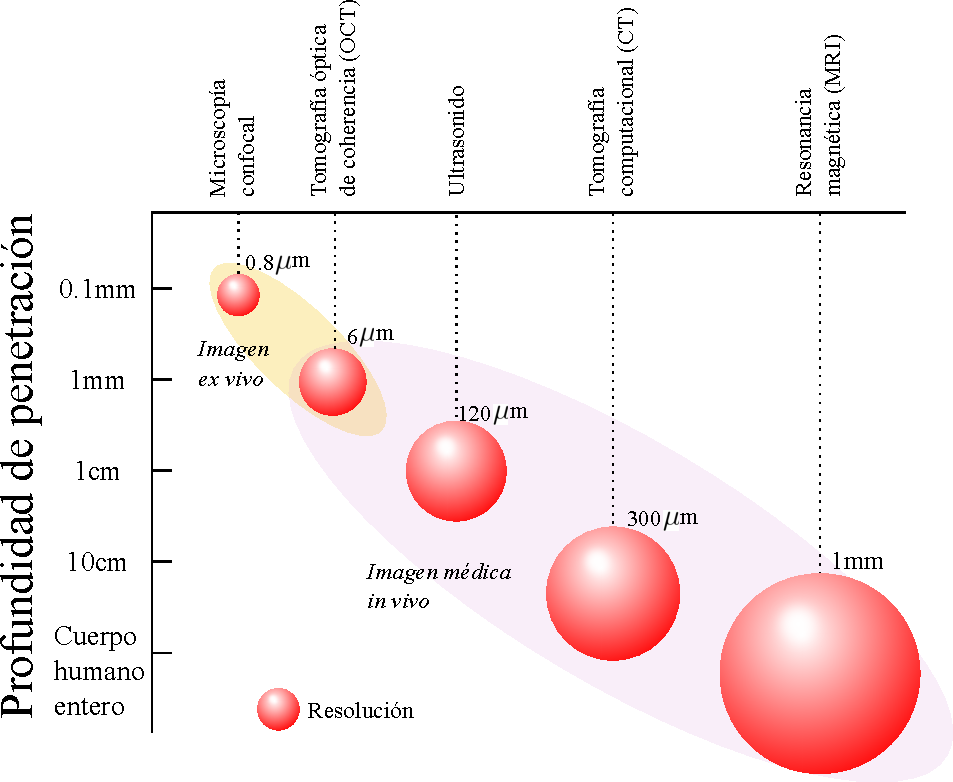
\includegraphics[width = 0.6\textwidth, keepaspectratio]{img/chap1/Carlos_oct_resolucion}
	\caption[Comparación de la resolución de distintas técnicas de imagen médica.]{Comparación de la resolución contra la profundidad de penetración de diferentes modalidades de imagen médica.}
	\label{fig:OCT_Ultrasound_microscopy}
\end{figure}

%La OCT es análoga al ultrasonido, con la diferencia de emplear luz en lugar de sonido. El principio básico de la OCT, es medir la magnitud y el retraso de las retrodipersiones o retroreflecciones de la luz en microestructuras en tejidos, de forma que el tamaño de las microsestructuras puede determinarse a través de la medida del tiempo que tarda el ``eco'' del sonido o la luz en viajar diferentes distancias. El desarrollo de equipos para tratamientos con ultrasonido a su vez ha posibilitado la creación de equipos de bajo costo para OCT, en especial si se considera que la velocidad del sonido es de alrededor de $1300m/s$, mientras que la luz viaja a $3\times 10^8 m/s$. Una de las principales ventajas de la analogía OCT/ultrasonido se encuentra en su fácil integración en instrumentos médicos, tales como catéteres, endoscopios, laparoscopios o incluso, agujas quirúrgicas que permite hacer imagen de órganos o tejidos sólidos \invivo en el cuerpo.



\section{Aplicaciones de OCT}

%\subsection{Los inicios de OCT}

%La propuesta de la técnica de OCT surgió hacia el año 1991 por Huang \etal \cite{Huang1991}, sus primeras pruebas fueron realizadas \emph{ex vivo} en la retina y la arteria coronaria. Huang \etal proponen una técnica análoga al ultrasonido, pero que en lugar de emplear ondas de sonido, emplea luz para realizar reconstrucciones tridimensionales a partir de escaneos bidimensionales, a esta técnica la denominarían tomografía óptica de coherencia, y se basa esencialmente en el empleo de un interferómetro de luz blanca. Con los resultados obtenidos por Huang \etal la OCT se ha posicionado como una de las más grandes aplicaciones emergentes para el diagnóstico oftalmológico e intravascular.

La propuesta de OCT surgió hacia el año 1991 por Huang \etal \cite{Huang1991}, sus primeras pruebas fueron realizadas \exvivo en la retina y la arteria coronaria, y desde estos resultados pudo verse la utilidad de OCT para el diagnóstico oftalmológico e intravascular, áreas en las que ha tenido grandes avances. El ojo humano puede ser analizado ópticamente, es decir, es posible implementar técnicas para observar de manera directa la zona interior del ojo, lo que ha impulsado el uso de métodos de imagen en oftalmología; muchos de los primeros estudios realizados con OCT fueron basados en el ojo humano. Las primeras imágenes \invivo de la retina fueron obtenidas de manera independiente por Fercher \etal \cite{Fercher1993} y Swanson \etal \cite{Swanson1993} en 1993. Estos resultados conllevaron a que en la década de los 90 se diera un alto uso de OCT para el monitoreo, seguimiento, detección y diagnosis de diferentes enfermedades, entre las cuales destaca: enfermedades maculares \cite{Puliafito1995}, incluyendo agujeros maculares \cite{Hee1995_2} y edemas maculares \cite{Hee1995},  coriorretinopatía serosa central \cite{Hee1995_3}, y degeneraciones maculares asociadas a la edad y a la neovascularización coroidal \cite{Hee1995_4}. Un ejemplo de monitoreo con OCT, está en el espesor de las capas de fibra del nervio retinal, el cual es un indicador de glaucoma, y que puede cuantificarse en ojos normales y con glaucoma. Mediante una correlación con medidas convencionales de la estructura y función del nervio óptico es posible encontrar focos de glaucoma, trabajo realizado también a partir de OCT en 1995 por Schuman \etal \cite{Schuman1995}.

La sensibilidad de OCT, en el orden de $-125dB$ o $10^{-12.5}$ veces la luz incidente, permite producir imagen de estructuras tales como la retina que poseen un bajo índice de esparcimiento, sin embargo, la mayor parte de las aplicaciones que emplean OCT requieren la captura de imágenes en tejidos que no son transparentes, y además, producen un alto esparcimiento y dispersión de la luz. En estos casos, es cuando la sensibilidad del método se vuelve relevante, ya que al ser la señal fuertemente atenuada por el esparcimiento, la sensibilidad es quien determina la profundidad hasta la cual se puede conseguir imágenes \cite{Drexler2015}. Las primeras imágenes de tejidos diferentes al ojo fueron posibles mediante el estudio de la influencia de la longitud de onda en el esparcimiento de la luz, en donde se obtuvo que longitudes de onda más largas que el visible reducen el esparcimiento producido por las muestras biológicas e incrementa la profundidad de penetración y la capacidad de producir imagen \cite{Brezinski1996, Schuman1995}. Uno de los primeros estudios del efecto de la longitud de onda sobre las reconstrucciones con OCT fue realizado por Brezinski \etal \cite{Brezinski1996}, quienes hicieron una comparación de imágenes capturadas a $850$ y $1300nm$ \exvivo en una epiglotis humana. La imagen tomada a $1300nm$ mostró una mayor penetración puesto que los principales absorbentes en la mayor parte de los tejidos son la melanina y la hemoglobina, los cuales poseen una alta absorción en el visible y el infrarrojo cercano \cite{Parsa1989}, mientras que la absorción del agua se convierte en dominante para mayores longitudes de onda, alrededor de los $1800-2000nm$. Por otro lado, en la mayoría de los tejidos, el esparcimiento en las longitudes de onda del infrarrojo cercano es uno o dos órdenes de magnitud mayores que la absorción, y éste disminuye para longitudes de onda más grandes.

%\begin{figure}[ht!]
%\centering
%\includegraphics[width = \textwidth, keepaspectratio]{img/oct_longitudes_multiples.png}
%\caption[OCT empleando diferentes longitudes de onda.]{Profundidad de penetración de la OCT en diferentes longitudes de onda. Comparación de la atenuación producida por diferentes longitudes de onda en OCT, visualmente se aprecian más detalles cuando se emplea una longitud de onda de $1300nm$ que con $850nm$. Tomado de \cite{Brezinski1996}.}
%\label{fig:oct_longitudes_multiples}
%\end{figure}

Muchos estudios iniciales de OCT se realizaron \exvivo en especímenes quirúrgicos, estos estudios fueron útiles para definir las estructuras que serían posibles de observar usando OCT \cite{Brezinski1996} y compararlo con la histología. El estudio de la correlación entre las imágenes \exvivo de OCT y la histología se extendió a hasta enfermedades gastrointestinales \cite{Izatt1996, Tearney1997, Kobayashi1998, Pitris2000}, biliares \cite{Tearney1998}, en el aparato reproductor femenino \cite{Pitris1999}, pulmonares \cite{Pitris1998} y urinarias \cite{Tearney1997}.



Los inicios de OCT fueron en oftalmología y hoy en día es una de las áreas con mayor impacto de esta técnica. OCT ha mostrado ser una herramienta bastante útil porque puede identificar característica de enfermedades desde etapas tempranas, permitiendo que se puedan realizar los tratamientos respectivos para prevenir el desarrollo de dichas enfermedades. Además, si se realizan tratamientos periódicos, puede mantenerse un monitoreo de la evolución de la terapia o de la enfermedad. OCT se ha convertido en una técnica importante para el diagnóstico y monitoreo de enfermedades tales como el glaucoma, la degeneración macular relacionada con la edad y la retinopatía diabética, ya que provee información cuantitativa de la patología lo que permite medir el progreso de la enfermedad o la respuesta ante terapias \cite{Hee1998, Schuman1995,Schuman1996}. Las imágenes de OCT proveen medidas cuantitativas de características tales como el espesor o el flujo sanguíneo, estas mediciones han derivado en otras aplicaciones relacionadas con OCT, tales como la obtención de mapas de espesor \cite{Hee1998}, lo que ha permitido generar estándares para la evaluación de algunas patologías presentes mediante la comparación con un estándar.

Otro ejemplo de implementación de OCT es la imagen intravascular. OCT ha permitido obtener imágenes que muestran de forma clara la diferencia entre la túnica íntima, la túnica media y la túnica adventicia al interior de las arterias \cite{Tearney1996_2}. En sus inicios, OCT intravascular \invivo representó un gran desafío, pues debían diseñarse catéteres apropiados para el uso en humanos, además de esto, dado que la sangre esparce altamente la luz, fue necesario la creación de un sistema de flujo para remover la sangre o para diluir los glóbulos rojos en el plano imagen. Los primeros estudios con OCT mediante endoscopios se realizaron en conejos por Fujimoto \etal en 1999 \cite{Fujimoto1999}, por otro lado, hacia el año 2001, Jang \emph{et al.} reportaron la primer imagen mediante OCT en pacientes humanos \cite{Jang2001}. El área intravascular representa una de las áreas actuales más activas en OCT, tanto desde un punto de vista comercial, como desde un punto de vista de investigación.

OCT también ha sido empleada en el caso de la endoscopia. El primer estudio de endoscopia \invivo con imágenes de OCT fue realizado en 1997 \cite{Tearney1997, Sergeev1997}, en donde se obtuvieron los primeros resultados para el análisis del esófago de un conejo. Las imágenes de OCT permitieron diferenciar de manera clara estructuras tales como la mucosa y la serosa. Los primeros estudios de endoscopia con imagen OCT en humanos fueron reportados por Sergeev \etal en 1997 \cite{Sergeev1997} y Feldchtein \etal en 1998 \cite{Feldchtein1998}, quienes mediante una sonda obtuvieron imágenes de membranas mucosas del esófago, la laringe, el estómago, la vejiga urinaria y el cuello uterino; mostrando así la utilidad de OCT en este tipo de imagen clínica.

Dado el crecimiento de casos de cáncer en el esófago, estomago y colon, la endoscopia gastrointestinal tuvo una mayor atención, en contraste con esto, los estudios iniciales de OCT mostraron las ventajas de esta técnica para visualizar estructuras superficiales, ya que permite ver no solo las capas exteriores, sino que adicionalmente puede observar morfologías de tejidos bajo la superficie, permitiendo diferenciar patologías gastrointestinales tales como el esófago de Barret, los pólipos adenomatosos y el adenocarcinoma \cite{Bouma1999, Sergeev1997, Rollins1999, Jackle2000, Jackle2000_2, Sivak2000}. Los estudios de OCT para detección de cáncer son complejos, ya que los resultados de OCT deben ser comparados con técnicas estandarizadas tales como la biopsia, el estándar en la detección de cáncer. El problema que tiene OCT es que el contraste producido por las variaciones en las propiedades esparsivas de diferentes tejidos puede producir errores en las muestras tomadas dada la sensibilidad de OCT.

Gracias a su alta sensibilidad y capacidad para producir imágenes volumétricas \emph{no-invasivas}, OCT ha sido de alto interés en diferentes áreas de la medicina, tales como la oftalmología \cite{Schuman1995, Swanson1993, Puliafito1995, Hee1995, Hee1995_2}, la imagen intravascular mediante catéteres \cite{Grube2002, Jang2002, Bouma2003}, la endoscopia \cite{Tearney1997,Feldchtein1998,Rollins1999}, la detección de cáncer \cite{Sergeev1997,Jackle2000}, la neurociencia \cite{Chen2009,Srinivasan2009,Lee2011}, la cardiología \cite{Li2012,Gu2012,Yazdanfar1997}, la dermatología \cite{Welzel1998,Gambichler2007,Blatter2012}, la odontología \cite{Otis2004,Melo2005,Bakhsh2011}, entre otras áreas.

\section{La investigación en OCT y la participación de América Latina}

Desde sus inicios, OCT ha visto un crecimiento exponencial en la cantidad de publicaciones por año sobre las diversas áreas de la medicina que abarca, así como los dispositivos y procedimientos con los que se realizan las imágenes. Como muestra de este crecimiento, solo en el año 2015 se estima que hubo 3500 publicaciones relacionadas con OCT \cite{Fujimoto2016}, como se muestra en la Fig.~\ref{fig:octpubbyyear}\footnote{Datos tomados de PUBMED.}. El área donde se realiza la mayor cantidad de publicaciones corresponde a oftalmología, seguida por el área cardiovascular y en tercer lugar, el desarrollo tecnológico, sin embargo, también desatacan otras áreas como la dermatología, odontología, neurología, entre otras. El gran desarrollo que ha tenido OCT está fuertemente relacionado con la aceptación a nivel clínico que ha tenido esta técnica, convirtiéndose en estándar para algunos procedimientos diagnósticos. En oftalmología, se estima que 30 millones de exámenes relacionados con OCT son realizados por año alrededor del mundo, y que aproximadamente 100 mil evaluaciones cardiovasculares por año son realizadas con OCT. 

\begin{figure}[ht!]
	\centering
	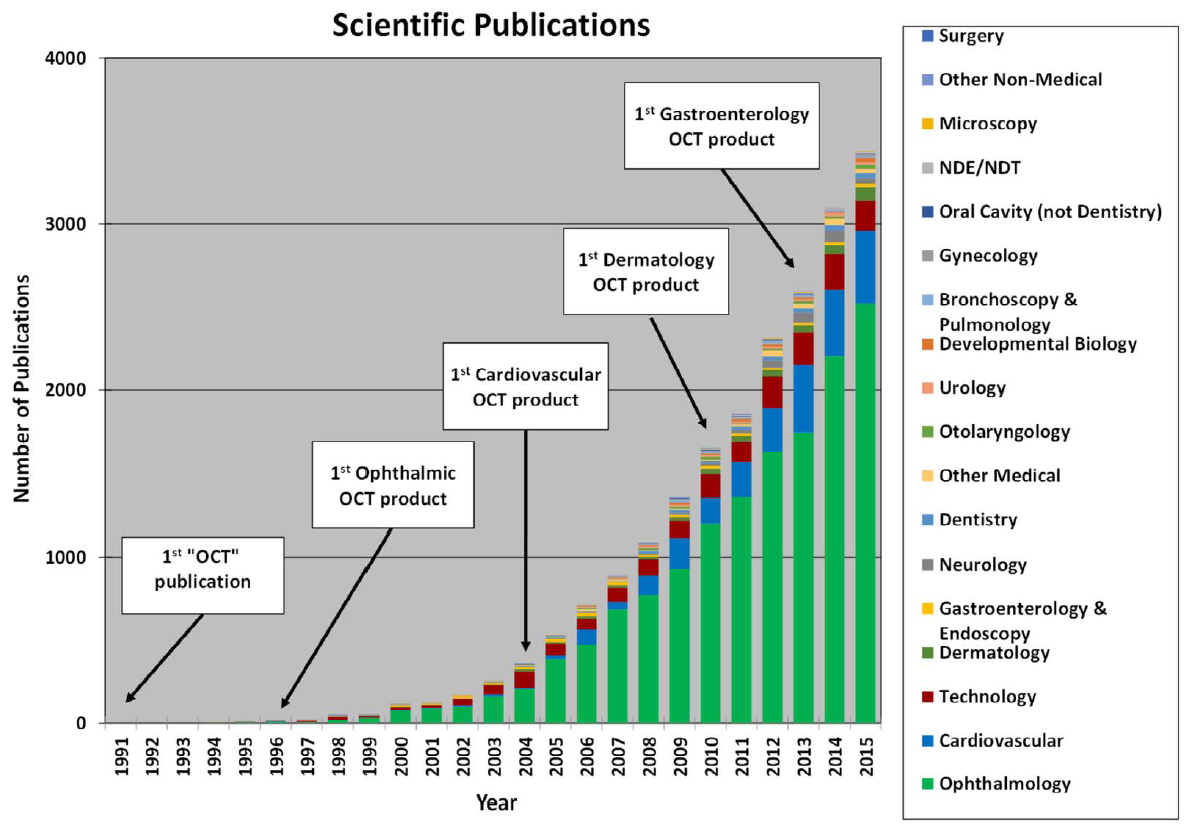
\includegraphics[width=0.7\linewidth]{img/chap1/oct_pub_by_year.png}
	\caption[Publicaciones de OCT por año.]{Publicaciones relacionadas con el desarrollo y aplicaciones de OCT por año. Oftalmología es la categoría más investigada, seguida por el área cardiovascular, y los dispositivos y técnicas en tercer lugar.}
	\label{fig:octpubbyyear}
\end{figure}

El crecimiento exponencial de la cantidad de publicaciones relacionadas con OCT, también se debe a la creación de empresas que comercializan equipos especializados tanto para el diagnóstico como para investigación. OCT ha crecido como un mercado atractivo para diversas compañías de equipos ópticos a nivel mundial, como lo son Zeiss o Thorlabs. En este sentido, el mercado que mueve OCT se estima en unos 700 millones de dólares anuales, como se muestra en la Fig.~\ref{subfig:octmarket}. Por otro lado, el 75\% de las compañías que producen equipos para OCT han surgido como \textit{start-ups} de las universidades que lideran el desarrollo científico de OCT, entre ellas, MIT y Harvard. En la Fig.~\ref{subfig:octcompaniesa} se muestra el crecimiento de las compañías que comercializan productos para diagnóstico e investigación con OCT.

\begin{figure}[ht!]
	\centering
	\subfigure[Mercado estimado de la comercialización de equipos de OCT.]{\label{subfig:octmarket}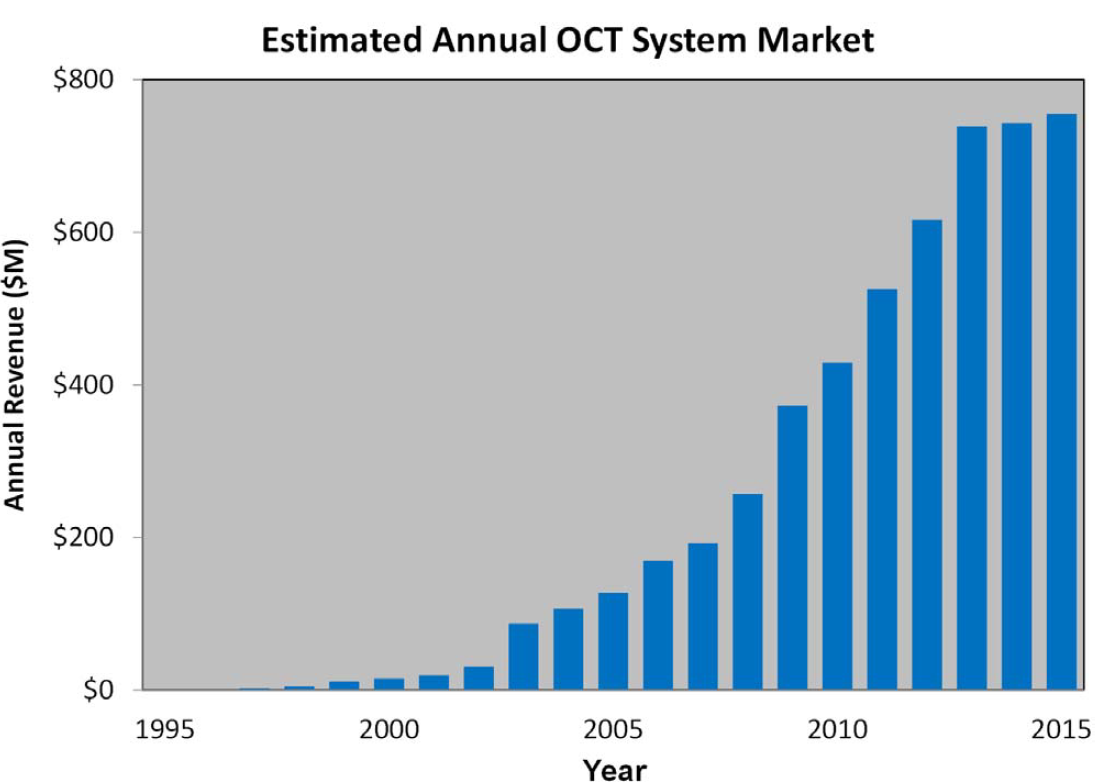
\includegraphics[width=0.45\linewidth]{img/chap1/oct_market}}
	\subfigure[Compañías relacionadas con equipos de OCT.]{\label{subfig:octcompaniesa}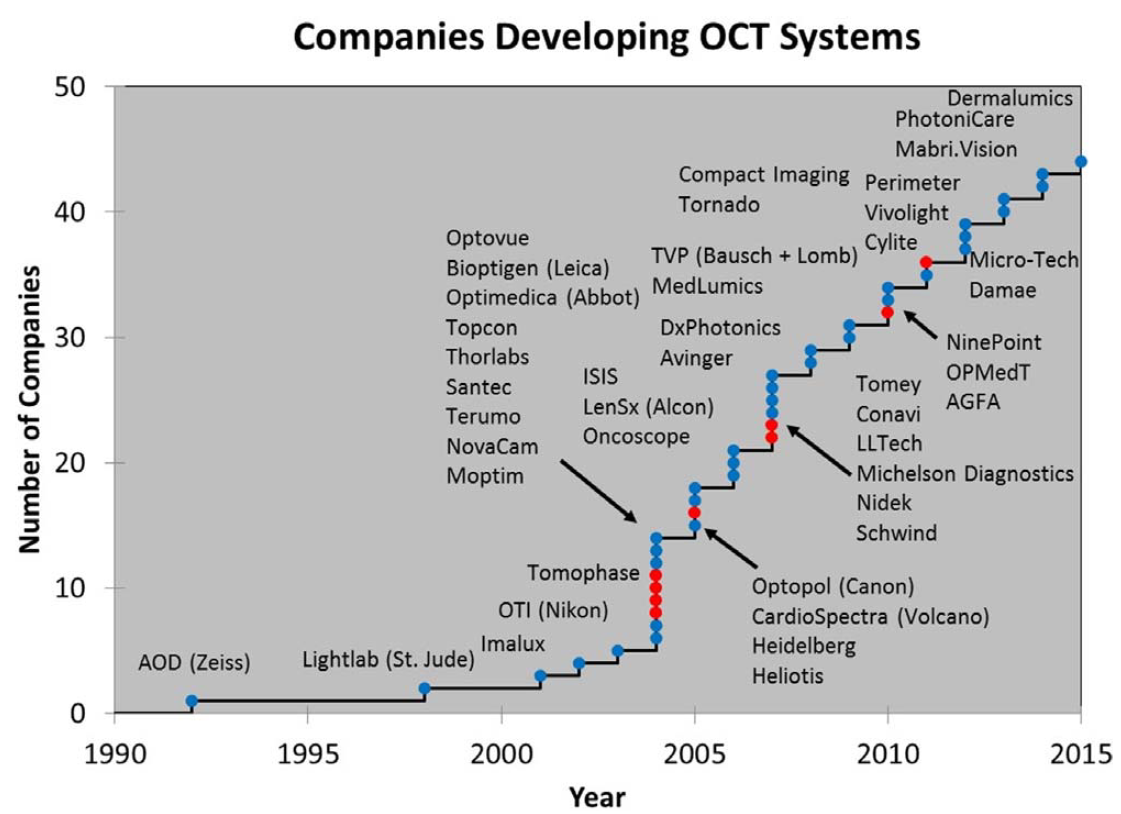
\includegraphics[width=0.45\linewidth]{img/chap1/oct_companiesa}}
	\caption[Mercado relacionado con OCT en los últimos años]{Mercado relacionado con OCT en los últimos años, hacia 2015 se estiman ingresos por $\approx700$ millones de dólares. La cantidad de compañías envueltas en OCT ha crecido a más de 45 en los últimos años, la mayor parte de estas han surgido como \textit{start-ups} provenientes de universidades (circulos azules).}
	\label{fig:octmarket}
\end{figure}

Aunque OCT ha tenido un crecimiento significativo en el ámbito médico e investigativo, cuando se analiza la participación de América Latina en este crecimiento, el panorama no es alentador. En la Fig.~\ref{fig:octgroups2015} se muestra un mapa de la colaboración entre grupos de investigación relacionados por el desarrollo científico en OCT en el año 2015. Los círculos negros representan la cantidad de grupos de investigación relacionados con el tema, mientras que las líneas grises que los une corresponde a la colaboración que hay entre grupos de investigación. En este mapa, se evidencia que a nivel de Latinoamérica, solamente Brasil cuenta con grupos de investigación trabajando en OCT, siendo la universidad de Coimbra (University of Coimbra), la más representativa. Aun con la gran comunidad internacional aportando a la investigación en OCT, no existe en la mayor parte de Latinoamérica, grupos de investigación que posean líneas de investigación relacionadas con OCT, esto a su vez está relacionado con la carencia de equipos especializados para el diagnóstico de enfermedades en donde OCT es el estándar. 

\begin{figure}[ht!]
	\centering
	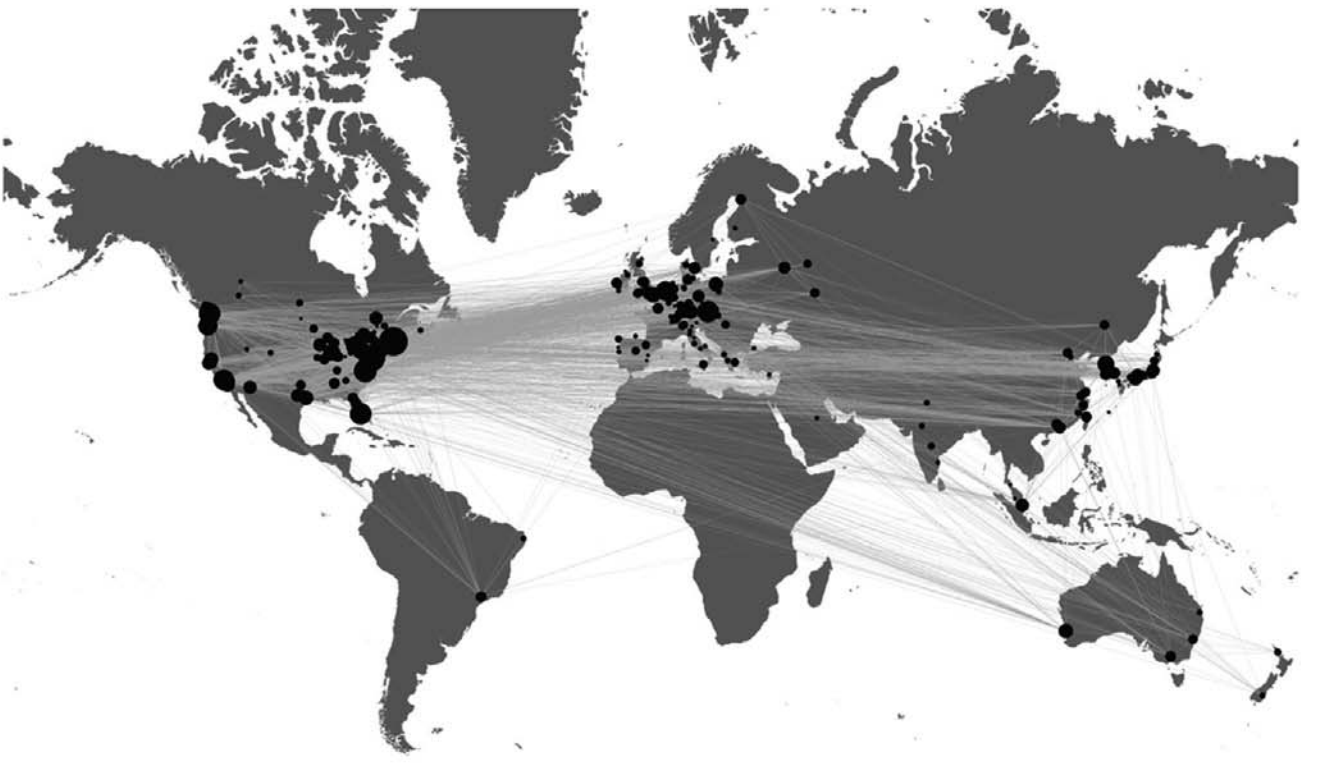
\includegraphics[width=0.7\linewidth]{img/chap1/oct_groups_2015}
	\caption[Mapa de grupos de investigación involucrados en OCT.]{Mapa de grupos de investigación con áreas afines a OCT con sus respectivas colaboraciones. En latinoamérica solo se cuenta con participación de Brasil.}
	\label{fig:octgroups2015}
\end{figure}




%\begin{figure*}
%	\centering
%	
%	\begin{subfigure}[b]{0.3\textwidth}
%		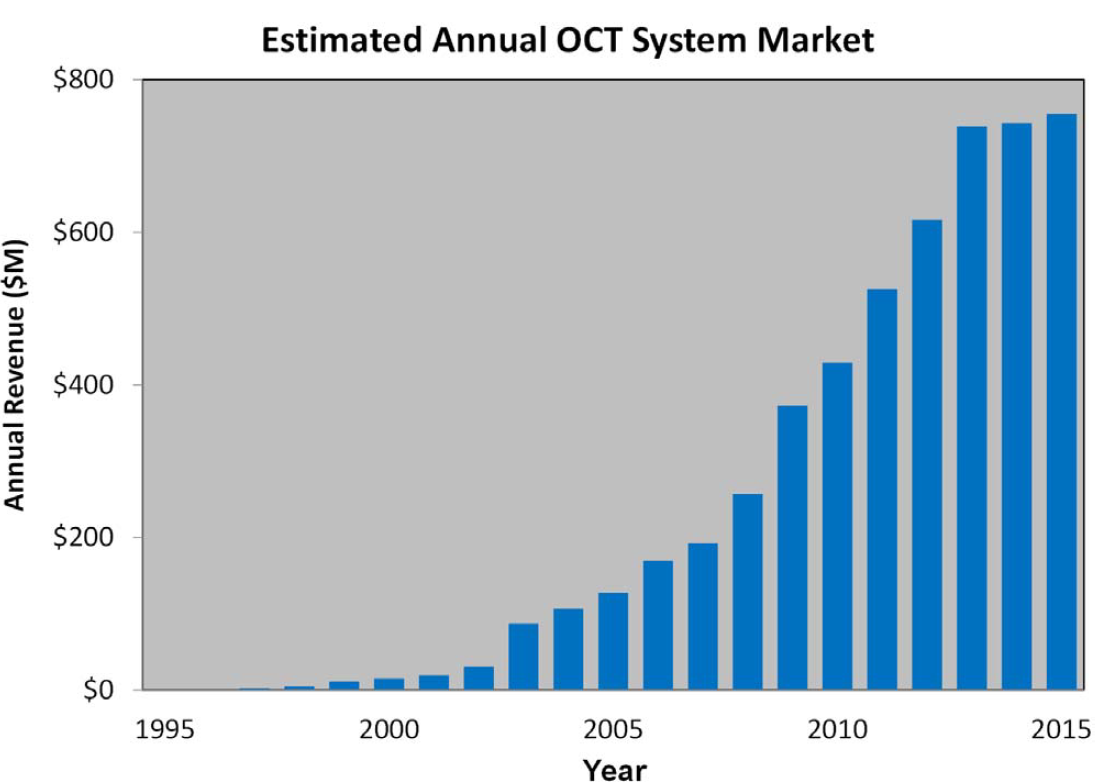
\includegraphics[width=0.4\linewidth]{img/chap1/oct_market}
%	\end{subfigure}%
%	~
%	\begin{subfigure}[b]{0.3\textwidth}
%		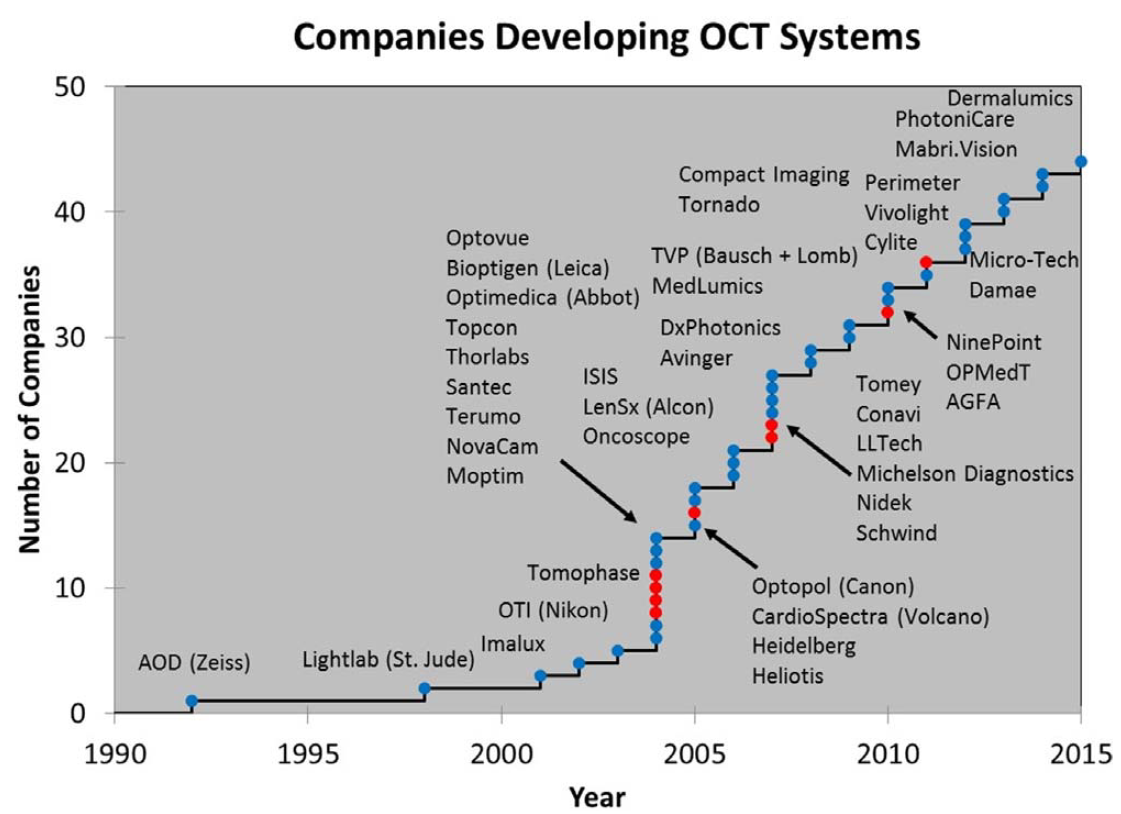
\includegraphics[width=0.4\linewidth]{img/chap1/oct_companiesa}
%	\end{subfigure}
%\end{figure*}


\section{Planteamiento del problema}
\label{sec:plant_problemo}
En la implementación inicial de OCT, la información en profundidad es obtenida mediante desplazamientos axiales del haz de referencia que son producidos por actuadores tales como piezoeléctricos, así como lo indica la Fig.~\ref{fig:scaningsystemoct}. En ese sistema de OCT, la luz producida por la fuente viaja mediante una fibra óptica hasta llegar a un acoplador, en donde se divide por dos caminos diferentes; uno de ellos viaja directamente hasta el espejo de referencia que tiene la posibilidad de desplazarse en sentido axial. Posteriormente, el haz reflejado por el espejo regresa hacia la fibra óptica. El segundo haz es dirigido hacia un espejo de escaneo cuya función es desviar la luz que es proyectada en la muestra de manera controlada. Mediante este sistema, la porción de luz que sea reflejada por la muestra hacia la fibra óptica volverá a incorporarse al sistema óptico regresando hasta el acoplador. La información de los dos haces juntos llega entonces hasta un sensor que se encarga de obtener la señal interferométrica. El sensor transfiere los datos a un sistema de adquisición de datos (DAQ) y finalmente las señales son enviadas hasta el computador. 

La información volumétrica requiere que el haz proyectado hacia la muestra sea desplazado de manera lateral en dos direcciones, procedimiento que se ha realizado a través del uso de sistemas microelectromecánicos (MEMS) que permiten la inclinación controlada del haz, y por tanto el desplazamiento de éste sobre la muestra \cite{Zara2003,Jung2006,Aguirre2007}. El espejo de escaneo se encarga de mover el haz sobre el plano imagen produciendo imágenes bidimensionales de planos $xy$ a profundidades $z$ específicas, a este tipo de imagen se le conoce como \emph{en-face}. Una de las limitaciones de los sistemas para OCT surge justamente en la implementación del sistema de escaneo, ya que hay errores producidos no solo por la instrumentación sino por la misma muestra. 

\begin{figure}[th!]
	\centering
	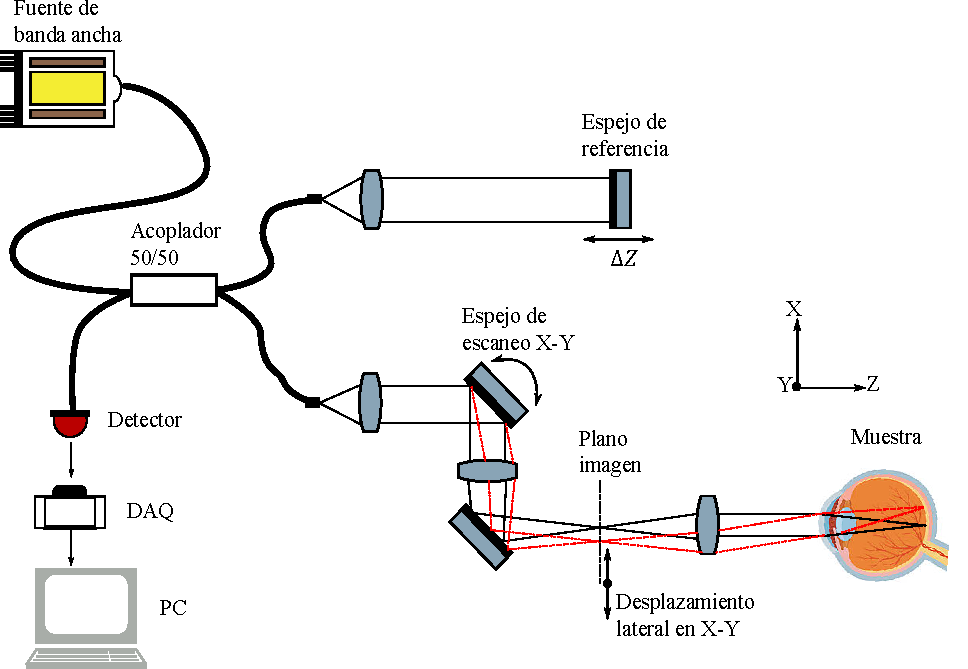
\includegraphics[width=0.7\linewidth]{img/chap1/scaning_system_oc.pdf}
	\caption[Esquema de un sistema de OCT]{Esquema de un sistema de escaneo de OCT para la retina.}
	\label{fig:scaningsystemoct}
\end{figure}


Desde el punto de vista instrumental, algunos espejos de escaneo emplean sistemas de control retroalimentados tales como PID que se encargan del desplazamiento y control del sistema \cite{xie2004}, sin embargo, este tipo de control en lazo cerrado puede tener la falencia de enviar voltajes fluctuantes  que producen desviaciones, y pueden ser causados o bien por las constantes del controlador o por desplazamientos repentinos producidos por el paciente. Otros sistemas basados en MEMS \cite{Strathman2014} requieren voltajes AC para producir respuestas lineales, sin embargo, fluctuaciones en la frecuencia o en la amplitud del voltaje suministrado al actuador producen respuestas diferentes a la esperada. Adicionalmente, mientras se realizan los escaneos axiales, el espejo de escaneo se mueve a velocidad constante en las dos direcciones, por lo tanto hay una dirección con una velocidad menor (\emph{slow-axis}) y otro con una mayor velocidad (\emph{fast-axis}), esto hace necesario una corrección del movimiento en las imágenes de OCT obtenidas \cite{Yun2004, Pierce2005, Drexler2015}. En cuanto a la muestra que es tomada en pacientes, existen diferentes movimientos involuntarios que no pueden ser controlados, tales como la contracción muscular causada por la respiración o el parpadeo, así como cualquier movimiento que el paciente pudiera realizar mientras el sistema se encuentra en proceso de escaneo.

%Las limitaciones mencionadas anteriormente, si bien pueden no tener una incidencia directa sobre la reconstrucción de la reflectividad producida por la muestra, si tiene un impacto directo en la reconstrucción de la fase, a estos errores en la fase las denominaremos corrupciones de fase. Ahora bien, como se ha mencionado, la OCT se basa en la medición de la interferencia causada entre la luz dispersada por una muestra y un haz de referencia \cite{Huang1991}. Bajo este principio, la OCT es capaz de medir no solo la amplitud del campo reflejado por la muestra, sino que también puede medir su fase; tomando esto en cuenta, numerosas extensiones de OCT que emplean principalmente la fase han surgido bajo el nombre de \emph{phase resolved OCT}, entre estas sobresalen: OCT Doppler \cite{Chen1999}, microangiografía óptica \cite{Wang2010}, elastografía óptica de coherencia \cite{Ruikang2007} y OCT magnetomotriz \cite{Oldenburg2005}. En OCT Doppler por ejemplo, es común encontrar aplicaciones de flujometría, en el cual el sistema interferométrico de la OCT permite la detección de saltos en la fase causados por el movimiento de los centros dispersores en la muestra que no es posible observar con la amplitud. Mediante este proceso, es posible seguir el movimiento de los centros dispersores y cuantificar su velocidad de flujo \cite{Chen1999}. 

Ahora bien, como se ha mencionado, OCT se basa en la medición de la interferencia causada entre la luz dispersada por una muestra y un haz de referencia \cite{Huang1991}. Bajo este principio, OCT es capaz de medir no solo la amplitud del campo reflejado por la muestra, sino que también puede medir su fase. Los errores en la toma de datos que pueden ser producidos por el sistema de escaneo así como el paciente, si bien pueden no tener una incidencia directa sobre la reconstrucción de la reflectividad de la muestra, si tiene un impacto directo en la reconstrucción de la fase. Numerosas extensiones de OCT que emplean principalmente la fase han surgido bajo el nombre de \emph{phase resolved OCT}, entre estas sobresalen: OCT Doppler \cite{Chen1999}, microangiografía óptica \cite{Wang2010}, elastografía óptica de coherencia \cite{Ruikang2007} y OCT magnetomotriz \cite{Oldenburg2005}. En OCT Doppler por ejemplo, es común encontrar aplicaciones de flujometría, en el cual el sistema interferométrico de OCT permite la detección de saltos en la fase causados por el movimiento de los centros dispersores en la muestra que no es posible observar con la amplitud. Mediante este proceso, es posible seguir el movimiento de los centros dispersores y cuantificar su velocidad de flujo \cite{Chen1999}. 

Otro problema que es común en los datos adquiridos mediante OCT es el moteado (\textit{speckle}), el cual cumple una doble función ya que puede aportar información de la muestra o puede surgir como ruido \cite{Schmitt1999,Mariampillai2008}. En OCT el \speckle como ruido surge cuando la señal que se registra en el detector posee información de la interferencia que se produce entre la luz dispersada por centros dispersores cercanos al área de escaneo, y en lugar de portar información sobre la muestra, degradan la calidad de la señal que se registra y dificultan su interpretación. En OCT existen diferentes técnicas de reducción de ruido multiplicativo causado por el \speckle \cite{Hughes2009,Szkulmowski2012,Aum2015}, aunque tienen la desventaja de poseer altos tiempos de procesamiento, y en algunos casos, requieren una imagen con bajo coeficiente señal-ruido para su correcto funcionamiento \cite{Fang2012}.

La propuesta para esta tesis de maestría consiste en facilitar la interpretación y procesamiento de datos provenientes de OCT, mediante la implementación de técnicas de posprocesamiento que permitan mejorar la calidad de los datos adquiridos, planteando posibles soluciones a algunos de los problemas mencionados anteriormente. 

La primera parte del trabajo de grado está orientado a la implementación de los conceptos básicos de OCT para recrear un sistema óptico que permite analizar muestras \textit{ex-vivo}. En el montaje experimental se obtuvo una resolución axial de $\approx2\mu m$ y una resolución lateral de $\approx3 \mu m$, con un escaneo máximo de $\approx1.5mm$ en profundidad y $\approx2.5mm$ de manera lateral, lo que permitió analizar muestras como monedas. Sin embargo, pese a las regulaciones existentes para el análisis \textit{in-vivo}, el montaje se probó en aplicaciones no médicas de OCT. Las primeras pruebas se realizaron en el escaneo de la topografía de una moneda, en donde se obtuvo una reconstrucción detallada del relieve que esta posee, las mediciones indicaron alturas máximas de $\approx50\mu m$. La segunda muestra que se estudió fue el ala frontal de un insecto \textit{ex-vivo}, donde se pudieron observar estructuras internas tales como la membrana. En este caso, se midió el espesor de la membrana, obteniéndose $\approx5\mu m$.

En la segunda parte del trabajo de grado, se planteó un nuevo método de filtrado de ruido por \speckle a partir del conocimiento de las causas y las características que éste posee, tomando elementos de técnicas de filtrado proveniente de las imágenes de radares de apertura sintética SAR. El algoritmo, conocido como \textit{non-loca means} (\textit{nlmeans}) fue planteado para el caso de ruido blanco, y gracias a sus resultados, ha sido extendido a diversas técnicas de imagen, entre ellas, imágenes SAR, en donde la obtención de los datos hace que también se de la presencia de ruido por \textit{speckle}. Modificando el funcionamiento de \nlmeans en el caso de ruido por \speckle y considerando las características de los datos disponibles en OCT, se propuso una modificación a \nlmeans denotada como \textit{NL-Means-OCT}. En \nlmeansOCT hay una combinación de los conceptos tradicionales de \nlmeans junto con otras implementaciones tridimensionales, lo que convierte a \nlmeansOCT en una herramienta útil para filtrar datos de OCT en donde es necesario la preservación de estructuras finas, o que se encuentran alteradas por la presencia de desplazamientos producidos por el paciente. Los resultados del filtrado con \nlmeansOCT mostraron conservar la fidelidad en la imagen mientras se elimina el ruido por \textit{speckle}. Dadas las características de \nlmeansOCT se pudo implementar de manera satisfactoria en otras áreas en desarrollo de OCT, entre ellas tractografía y gastroenterología.

La última parte del trabajo consistió en el planteamiento de un nuevo método para la corrección de problemas en la fase de un sistema de OCT a partir de fuente de barrido. El problema de la fase surge porque la fuente de barrido tiene fluctuaciones de sincronía con el fotodetector, por lo que la fase del tomograma puede sufrir alteraciones. En vista de que son pocos los algoritmos existentes para abordar este problema, se planteó un método de solución a partir de una optimización, tomando como función objetivo los espectros de potencia asociados con el tomograma, de manera que el espectro de potencia del tomograma afectado se aproxima al de un tomograma ideal mediante una minimización. Aplicando conceptos del enfoque en medios turbios, la implementación muestra encontrar de manera satisfactoria los mapas de corrupción en la fase. Las simulaciones indican que el algoritmo puede encontrar una buena representación del mapa de corrupción real a partir de la aproximación de valores mediante una función de mérito. Los resultados experimentales preliminares verifican la hipótesis de que este modelo mejora los planteamientos actuales de otros autores.

\section{Objetivos}

\subsection{Objetivo General}
%Desarrollar métodos de optimización en paralelo para la identificación de objetos de fase para la tomografía óptica coherente para diagnosis médico.
%Mejorar la identificación de objetos de fase en tomografía óptica coherente mediante optimización en paralelo, que ayuden en el diagnosis médico.
Estabilizar la fase en tomografía óptica de coherencia mediante posprocesamiento.

\subsection{Objetivos Específicos}

\begin{itemize}
	\item Identificar el estado de arte de la tomografía óptica de coherencia en aplicaciones biomédicas.
	%	\item Implementar un sistema óptico equivalente a los montajes utilizados durante la primera generación de la tomografía óptica coherente.
	\item Implementar un sistema óptico de prueba de concepto de campo completo en la tomografía óptica de coherencia.
	%	\item Simular un volumen de datos que represente un objeto característico encontrados en la tomografía óptica coherente.
	%	\item Simular un volumen de datos que posea las características de los objetos que se pueden encontrar en la tomografía óptica coherente, incluyendo las corrupciones de fase provenientes del muestreo.
	\item Realizar una simulación del muestreo y la formación de imagen en la tomografía óptica de coherencia, incluyendo elementos de corrupción de fase.
	%	\item Desarrollar y aplicar un método de optimización de fase que permita encontrar las características del objeto simulado anteriormente.
	\item Desarrollar un método de posprocesamiento que permita recuperar el mapa de corrupción de la imagen simulada anteriormente.
	%	\item Definir una métrica del error para evaluar la convergencia del algoritmo de optimización propuesto.
	\item Comprobar experimentalmente la funcionalidad del algoritmo propuesto con datos experimentales suministrados por el \emph{Wellman Center for Photomedicine, Harvard Medical School and Massachusetts General Hospital}.
	
\end{itemize}

\section{Estructura del documento, descripción de los objetivos y resultados esperados}

El documento se encuentra dividido en cinco capítulos en los cuales se abordarán los objetivos específicos del trabajo de grado. El primer objetivo, relacionado con la generación de un estado del arte de los avances en los que OCT se ha visto involucrado, se encuentra distribuido entre el Capítulo~\ref{chapter:intro} y las primeras secciones del Capítulo~\ref{chapter:aspectos_teo_y_pract_oct}. En el Capítulo~\ref{chapter:intro} se ha mostrado la relación que tiene OCT con la medicina, la investigación en torno a OCT y la importancia que reviste actualmente, en adición a esto, se optó por abordar fundamentos y conceptos básicos de la física que se aplican en OCT como parte del estado del arte, esto será discutido en el Capítulo~\ref{chapter:aspectos_teo_y_pract_oct}. El resultado que se espera de entender los conceptos de OCT, es la implementación de un sistema a nivel de laboratorio que permita aplicar sus fundamentos y enfrentar los retos que tiene cualquier equipo de OCT durante su desarrollo. Como consecuencia de esto, el segundo objetivo, asociado con un sistema óptico de prueba de concepto se describirá en el Capítulo~\ref{chapter:aspectos_teo_y_pract_oct}, en donde se mostrarán los detalles del montaje, las pruebas realizadas y los resultados obtenidos.

La segunda parte del trabajo de grado fue orientado a la aplicación de métodos de posprocesamiento que permitan abordar problemas presentes en OCT como los mencionados en el planteamiento del problema (Sección~\ref{sec:plant_problemo}), en ese orden de ideas, en el trabajo de grado se trataron dos problemas relacionados con la fase en OCT, siendo estos, el ruido por \speckle y la distorsión en la fase por falta de sincronía en OCT. Los tres últimos objetivos del trabajo de grado, se encuentran entonces distribuidos en los Capítulos \ref{chapter:supresion_ruido_en_oct} y \ref{chapter:estabilizacion_fase}, en donde se abordarán los dos temas mencionados anteriormente en su respectivo orden.

En el Capítulo \ref{chapter:supresion_ruido_en_oct} se analizarán las causas y características que tiene el \speckle  que se produce en OCT, y se planteará una técnica de filtrado que permite emplear de manera más efectiva la información disponible en OCT para suprimir el ruido por \textit{speckle}. En este capítulo se abordará parte de los objetivos cuatro y cinco, pues se propondrá una técnica de posprocesamiento que permite corregir uno de los problemas de OCT relacionado con la fase, entendiendo que la corrupción en este caso es ocasionada por el ruido de \text{speckle}. De este método de filtrado se obtuvo una aplicación multidisciplinar en OCT, ya que dadas sus características es de implementación directa en otras áreas derivadas de OCT.

En el Capítulo \ref{chapter:estabilizacion_fase} se tratará un problema que surge en OCT por las limitaciones que tienen los equipos que se emplean en los sistemas de alta velocidad, en donde la fase medida puede verse alterada por falta de sincronía en los equipos. Este capítulo aborda el objetivo tres, y la parte final de los objetivos cuatro y cinco del trabajo de grado. En este caso, se planteará un método de posprocesamiento que permite corregir la fase de un tomograma a partir de una optimización, conociendo las características que originan el problema. El producto final que se espera, es obtener fases en donde se compensen los inconvenientes de la instrumentación mediante la técnica propuesta.

En el capítulo \ref{chapter:conclusiones} se refrendarán los objetivos del trabajo de grado con respecto a las implementaciones y resultados obtenidos. Asimismo, se resumirán brevemente las ventajas de los procedimiento propuesto, y se planteará el trabajo futuro para la línea de OCT que se ha desarrollado. 


\bibliographystyle{unsrt}
\bibliography{ref/Ref_chap_1}